\documentclass{article}
\usepackage[utf8]{inputenc}
\usepackage{geometry}
\usepackage{amsmath}
\usepackage{amssymb}
\usepackage{enumitem}
\usepackage{graphicx}
\usepackage{multicol}
\graphicspath{ {../images/} }

\geometry{letterpaper, margin=1in}

\begin{document}

\begin{center}
    {\LARGE EE114 - Homework 1} \\[0.5cm]
    Name: Kaushik Vada \\[0.5cm]
    \today
\end{center}

\section*{Quiz 1.1}
\begin{minipage}{0.65\textwidth}
    A pizza at Gerlanda's is either regular ($R$) or Tuscan ($T$). In addition, each slice may have mushrooms ($M$) or onions ($O$) as described by the Venn diagram at right. For the sets specified below, shade the corresponding region of the Venn diagram.
    \begin{multicols}{2}
        \begin{enumerate}[label=(\arabic*)]
            \item $R$ \\ {\boldmath\textbf{Regular pizzas (outside T)}}
            \item $M \cap O$ \\ {\boldmath\textbf{Mushrooms AND Onions (overlap)}}
            \item $R \cap M$ \\ {\boldmath\textbf{Regular AND Mushrooms (overlap M and R)}}
            \item $M \cup O$ \\ {\boldmath\textbf{Mushrooms OR Onions (union)}}
            \item $R \cup M$ \\ {\boldmath\textbf{Regular OR Mushrooms (union)}}
            \item $T^c - M$ \\ {\boldmath\textbf{Not Tuscan minus Mushrooms (Regular sans M)}}
        \end{enumerate}
    \end{multicols}
\end{minipage}
\hfill
\begin{minipage}{0.3\textwidth}
    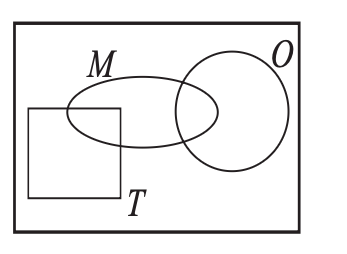
\includegraphics[width=\textwidth]{quiz_1_1.png}
\end{minipage}

\section*{Problem 1.1.1}
For Gerlanda's pizza in Quiz 1.1, answer these questions:
\begin{enumerate}[label=(\alph*)]
    \item Are $T$ and $M$ mutually exclusive? \\
    {\boldmath\textbf{No. The Venn diagram shows that the set $M$ (mushrooms) overlaps with the set $T$ (Tuscan), meaning it is possible to have a Tuscan pizza with mushrooms. No, they are not mutually exclusive.}}
    
    \item Are $R, T,$ and $M$ collectively exhaustive? \\
    {\boldmath\textbf{Yes. Since $R$ and $T$ represent all possible pizza types (Regular and Tuscan) and form a partition of the space (assuming every pizza is either R or T), the union $R \cup T$ is the entire sample space. Adding $M$ doesn't change this coverage. Yes, they are collectively exhaustive.}}
    
    \item Are $T$ and $O$ mutually exclusive? State this condition in words. \\
    {\boldmath\textbf{The diagram shows $O$ (onions) overlaps with $T$ (Tuscan). Thus, they are not mutually exclusive. No. Words: One can order a Tuscan pizza with onions.}}
    
    \item Does Gerlanda's make Tuscan pizzas with mushrooms and onions? \\
    {\boldmath\textbf{This asks if $T \cap M \cap O$ is non-empty. Based on the intersection of the $M$ and $O$ circles within the $T$ region: Yes.}}
    
    \item Does Gerlanda's make regular pizzas that have neither mushrooms nor onions? \\
    {\boldmath\textbf{This asks if $R \cap M^c \cap O^c$ is non-empty. This corresponds to the region inside $R$ but outside both $M$ and $O$. Yes.}}
\end{enumerate}

\newpage

\section*{Problem 1.2.1}
A fax transmission can take place at any of three speeds depending on the condition of the phone connection between the two fax machines. The speeds are high ($h$) at 14,400 b/s, medium ($m$) at 9600 b/s, and low ($l$) at 4800 b/s. In response to requests for information, a company sends either short faxes of two ($t$) pages, or long faxes of four ($f$) pages. Consider the experiment of monitoring a fax transmission and observing the transmission speed and length. An observation is a two-letter word, for example, a high-speed, two-page fax is $ht$.

\begin{enumerate}[label=(\alph*)]
    \item What is the sample space of the experiment? \\
    {\boldmath\textbf{The sample space consists of all pairs of speed $S \in \{h, m, l\}$ and length $L \in \{t, f\}$: S = \{ht, hf, mt, mf, lt, lf\}}}
    
    \item Let $A_1$ be the event ``medium-speed fax.'' What are the outcomes in $A_1$? \\
    {\boldmath\textbf{$A_1$ includes all outcomes where the speed is $m$: $\mathbf{A_1} = \{mt, mf\}$}}
    
    \item Let $A_2$ be the event ``short (two-page) fax.'' What are the outcomes in $A_2$? \\
    {\boldmath\textbf{$A_2$ includes all outcomes where the length is $t$: $\mathbf{A_2} = \{ht, mt, lt\}$}}
    
    \item Let $A_3$ be the event ``high-speed fax or low-speed fax.'' What are the outcomes in $A_3$? \\
    {\boldmath\textbf{$A_3$ includes outcomes where speed is $h$ or $l$: $\mathbf{A_3} = \{ht, hf, lt, lf\}$}}
    
    \item Are $A_1, A_2,$ and $A_3$ mutually exclusive? \\
    {\boldmath\textbf{Check intersection $A_1 \cap A_2 = \{mt\}$. Since the intersection is not empty, they are not mutually exclusive. No.}}
    
    \item Are $A_1, A_2,$ and $A_3$ collectively exhaustive? \\
    {\boldmath\textbf{The union $A_1 \cup A_2 \cup A_3 = \{mt, mf\} \cup \{ht, mt, lt\} \cup \{ht, hf, lt, lf\}$. Any outcome in $S$ is present in at least one set. Yes.}}
\end{enumerate}

\newpage

\section*{Problem 1.2.2}
An integrated circuit factory has three machines $X, Y,$ and $Z$. Test one integrated circuit produced by each machine. Either a circuit is acceptable ($a$) or it fails ($f$). An observation is a sequence of three test results corresponding to the circuits from machines $X, Y,$ and $Z$, respectively. For example, $aaf$ is the observation that the circuits from $X$ and $Y$ pass the test and the circuit from $Z$ fails the test.

\begin{enumerate}[label=(\alph*)]
    \item What are the elements of the sample space of this experiment? \\
    {\boldmath\textbf{Each machine has 2 outcomes ($a, f$). Total outcomes $2^3 = 8$. S = \{aaa, aaf, afa, aff, faa, faf, ffa, fff\}}}
    
    \item What are the elements of the sets
    \[ Z_F = \{ \text{circuit from } Z \text{ fails} \}, \]
    \[ X_A = \{ \text{circuit from } X \text{ is acceptable} \}. \]
    {\boldmath\textbf{$Z_F$ are outcomes ending in $f$: $\mathbf{Z_F} = \{aaf, aff, faf, fff\}$}} \\
    {\boldmath\textbf{$X_A$ are outcomes starting with $a$: $\mathbf{X_A} = \{aaa, aaf, afa, aff\}$}}
    
    \item Are $Z_F$ and $X_A$ mutually exclusive? \\
    {\boldmath\textbf{The intersection $Z_F \cap X_A = \{aaf, aff\}$. Since it is not empty: No.}}
    
    \item Are $Z_F$ and $X_A$ collectively exhaustive? \\
    {\boldmath\textbf{The union $Z_F \cup X_A = \{aaa, aaf, afa, aff, faf, fff\}$. Missing outcomes $\{faa, ffa\}$. No.}}
    
    \item What are the elements of the sets
    \[ C = \{ \text{more than one circuit acceptable} \}, \]
    \[ D = \{ \text{at least two circuits fail} \}. \]
    {\boldmath\textbf{$C = \{2 \text{ or } 3 \text{ a's} \}$: $\mathbf{C} = \{aaa, aaf, afa, faa\}$}} \\
    {\boldmath\textbf{$D = \{2 \text{ or } 3 \text{ f's} \}$: $\mathbf{D} = \{aff, faf, ffa, fff\}$}}
    
    \item Are $C$ and $D$ mutually exclusive? \\
    {\boldmath\textbf{An outcome cannot have $\ge 2$ a's and $\ge 2$ f's simultaneously in length 3. Yes.}}
    
    \item Are $C$ and $D$ collectively exhaustive? \\
    {\boldmath\textbf{Every outcome has either fewer than 2 f's (so $\ge 2$ a's) or $\ge 2$ f's. The union covers all 8 outcomes. Yes.}}
\end{enumerate}

\newpage

\section*{Problem 1.3.1}
Computer programs are classified by the length of the source code and by the execution time. Programs with more than 150 lines in the source code are big ($B$). Programs with $\le 150$ lines are little ($L$). Fast programs ($F$) run in less than 0.1 seconds. Slow programs ($W$) require at least 0.1 seconds. Monitor a program executed by a computer. Observe the length of the source code and the run time. The probability model for this experiment contains the following information: $P[LF] = 0.5$, $P[BF] = 0.2$, and $P[BW] = 0.2$. What is the sample space of the experiment? Calculate the following probabilities:

{\boldmath\textbf{Sample space is \{LF, LW, BF, BW\}. We can calculate $P[LW] = 1 - (0.5+0.2+0.2) = 0.1$.}}

\begin{enumerate}[label=(\alph*)]
    \item $P[W]$ \\
    {\boldmath\textbf{$P[W] = P[LW] + P[BW] = 0.1 + 0.2 = 0.3$}}
    
    \item $P[B]$ \\
    {\boldmath\textbf{$P[B] = P[BF] + P[BW] = 0.2 + 0.2 = 0.4$}}
    
    \item $P[W \cup B]$ \\
    {\boldmath\textbf{$P[W \cup B] = P[LW] + P[BW] + P[BF] = 0.1 + 0.2 + 0.2 = 0.5$}}
\end{enumerate}

\newpage

\section*{Problem 1.3.2}
There are two types of cellular phones, handheld phones ($H$) that you carry and mobile phones ($M$) that are mounted in vehicles. Phone calls can be classified by the traveling speed of the user as fast ($F$) or slow ($W$). Monitor a cellular phone call and observe the type of telephone and the speed of the user. The probability model for this experiment has the following information: $P[F] = 0.5$, $P[HF] = 0.2$, $P[MW] = 0.1$. What is the sample space of the experiment? Calculate the following probabilities:

{\boldmath\textbf{Sample space is \{HF, HW, MF, MW\}.
We deduce $P[MF] = P[F] - P[HF] = 0.5 - 0.2 = 0.3$.
Summing all probabilities: $P[HW] = 1 - (0.2 + 0.3 + 0.1) = 0.4$.}}

\begin{enumerate}[label=(\alph*)]
    \item $P[W]$ \\
    {\boldmath\textbf{$P[W] = P[HW] + P[MW] = 0.4 + 0.1 = 0.5$}}
    
    \item $P[MF]$ \\
    {\boldmath\textbf{From above: 0.3}}
    
    \item $P[H]$ \\
    {\boldmath\textbf{$P[H] = P[HF] + P[HW] = 0.2 + 0.4 = 0.6$}}
\end{enumerate}

\newpage

\section*{Problem 1.4.1}
Mobile telephones perform \textit{handoffs} as they move from cell to cell. During a call, a telephone either performs zero handoffs ($H_0$), one handoff ($H_1$), or more than one handoff ($H_2$). In addition, each call is either long ($L$), if it lasts more than three minutes, or brief ($B$). The following table describes the probabilities of the possible types of calls.

\begin{center}
\begin{tabular}{c|ccc}
 & $H_0$ & $H_1$ & $H_2$ \\
\hline
$L$ & 0.1 & 0.1 & 0.2 \\
$B$ & 0.4 & 0.1 & 0.1
\end{tabular}
\end{center}

\noindent
\noindent
What is the probability $P[H_0]$ that a phone makes no handoffs? \\
{\boldmath\textbf{$P[H_0] = 0.1 + 0.4 = 0.5$}}

\noindent
What is the probability a call is brief? \\
{\boldmath\textbf{$P[B] = 0.4 + 0.1 + 0.1 = 0.6$}}

\noindent
What is the probability a call is long or there are at least two handoffs? \\
{\boldmath\textbf{$P[L \cup H_2] = P[L] + P[H_2] - P[L \cap H_2] = 0.4 + 0.3 - 0.2 = 0.5$}}

\newpage

\section*{Problem 1.4.2}
For the telephone usage model of Example 1.14, let $B_m$ denote the event that a call is billed for $m$ minutes. To generate a phone bill, observe the duration of the call in integer minutes (rounding up). Charge for $M$ minutes $M = 1, 2, 3, \dots$ if the exact duration $T$ is $M - 1 < t \le M$. A more complete probability model shows that for $m = 1, 2, \dots$ the probability of each event $B_m$ is
\[ P[B_m] = \alpha(1 - \alpha)^{m-1} \]
where $\alpha = 1 - (0.57)^{1/3} = 0.171$.

\begin{enumerate}[label=(\alph*)]
    \item Classify a call as long, $L$, if the call lasts more than three minutes. What is $P[L]$? \\
    {\boldmath\textbf{$P[L] = P[M \ge 4] = \sum_{m=4}^\infty \alpha(1-\alpha)^{m-1} = (1-\alpha)^3 = (0.57^{1/3})^3 = 0.57$}}
    
    \item What is the probability that a call will be billed for nine minutes or less? \\
    {\boldmath\textbf{$P[M \le 9] = 1 - P[M > 9] = 1 - (1-\alpha)^9 = 1 - (0.57^{1/3})^9 = 1 - 0.57^3 \approx 0.815$}}
\end{enumerate}

\newpage

\section*{Problem 1.4.3}
The basic rules of genetics were discovered in mid-1800s by Mendel, who found that each characteristic of a pea plant, such as whether the seeds were green or yellow, is determined by two genes, one from each parent. Each gene is either dominant $d$ or recessive $r$. Mendel's experiment is to select a plant and observe whether the genes are both dominant $d$, both recessive $r$, or one of each (hybrid) $h$. In his pea plants, Mendel found that yellow seeds were a dominant trait over green seeds. A $yy$ pea with two yellow genes has yellow seeds; a $gg$ pea with two recessive genes has green seeds; a hybrid $gy$ or $yg$ pea has yellow seeds. In one of Mendel's experiments, he started with a parental generation in which half the pea plants were $yy$ and half the plants were $gg$. The two groups were crossbred so that each pea plant in the first generation was $gy$. In the second generation, each pea plant was equally likely to inherit a $y$ or a $g$ gene from each first generation parent. What is the probability $P[Y]$ that a randomly chosen pea plant in the second generation has yellow seeds?

{\boldmath\textbf{Each parent in Gen 1 is $Yg$. Offspring receives $Y$ or $g$ with prob 0.5 from each.
Outcomes for offspring genes: $YY, Yg, gY, gg$, each with prob $0.25$.
Yellow seeds occur for $\{YY, Yg, gY\}$.
$P[Y] = 0.25 + 0.25 + 0.25 = 0.75$}}

\newpage

\section*{Problem 1.4.4}
Use Theorem 1.7 to prove the following facts:
\begin{enumerate}[label=(\alph*)]
    \item $P[A \cup B] \ge P[A]$ \\
    {\boldmath\textbf{$A \cup B = A \cup (B \cap A^c)$, disjoint. $P[A \cup B] = P[A] + P[B \cap A^c]$. Since $P(\cdot) \ge 0$, proven.}}
    
    \item $P[A \cup B] \ge P[B]$ \\
    {\boldmath\textbf{Similarly, $P[A \cup B] = P[B] + P[A \cap B^c] \ge P[B]$. Proven.}}
    
    \item $P[A \cap B] \le P[A]$ \\
    {\boldmath\textbf{$A = (A \cap B) \cup (A \cap B^c)$. $P[A] = P[A \cap B] + P[A \cap B^c] \ge P[A \cap B]$. Proven.}}
    
    \item $P[A \cap B] \le P[B]$ \\
    {\boldmath\textbf{Similarly $P[B] \ge P[A \cap B]$. Proven.}}
\end{enumerate}

\newpage

\section*{Problem 1.4.5}
Use Theorem 1.7 to prove by induction the \textit{union bound}: For any collection of events $A_1, \dots, A_n$,
\[ P[A_1 \cup A_2 \cup \dots \cup A_n] \le \sum_{i=1}^n P[A_i]. \]

\noindent {\boldmath\textbf{Base case (n=2): $P[A_1 \cup A_2] = P[A_1] + P[A_2] - P[A_1 \cap A_2] \le P[A_1] + P[A_2]$.}} \\
{\boldmath\textbf{Inductive step: Assume for $k$. For $k+1$, let $B = \cup_{i=1}^k A_i$. \\
$P[B \cup A_{k+1}] \le P[B] + P[A_{k+1}] \le (\sum_{i=1}^k P[A_i]) + P[A_{k+1}]$. Proven.}}

\end{document}